% Options for packages loaded elsewhere
% Options for packages loaded elsewhere
\PassOptionsToPackage{unicode}{hyperref}
\PassOptionsToPackage{hyphens}{url}
\PassOptionsToPackage{dvipsnames,svgnames,x11names}{xcolor}
%
\documentclass[
  10pt,
  letterpaper,
  DIV=11,
  numbers=noendperiod]{scrartcl}
\usepackage{xcolor}
\usepackage{amsmath,amssymb}
\setcounter{secnumdepth}{5}
\usepackage{iftex}
\ifPDFTeX
  \usepackage[T1]{fontenc}
  \usepackage[utf8]{inputenc}
  \usepackage{textcomp} % provide euro and other symbols
\else % if luatex or xetex
  \usepackage{unicode-math} % this also loads fontspec
  \defaultfontfeatures{Scale=MatchLowercase}
  \defaultfontfeatures[\rmfamily]{Ligatures=TeX,Scale=1}
\fi
\usepackage{lmodern}
\ifPDFTeX\else
  % xetex/luatex font selection
\fi
% Use upquote if available, for straight quotes in verbatim environments
\IfFileExists{upquote.sty}{\usepackage{upquote}}{}
\IfFileExists{microtype.sty}{% use microtype if available
  \usepackage[]{microtype}
  \UseMicrotypeSet[protrusion]{basicmath} % disable protrusion for tt fonts
}{}
% Make \paragraph and \subparagraph free-standing
\makeatletter
\ifx\paragraph\undefined\else
  \let\oldparagraph\paragraph
  \renewcommand{\paragraph}{
    \@ifstar
      \xxxParagraphStar
      \xxxParagraphNoStar
  }
  \newcommand{\xxxParagraphStar}[1]{\oldparagraph*{#1}\mbox{}}
  \newcommand{\xxxParagraphNoStar}[1]{\oldparagraph{#1}\mbox{}}
\fi
\ifx\subparagraph\undefined\else
  \let\oldsubparagraph\subparagraph
  \renewcommand{\subparagraph}{
    \@ifstar
      \xxxSubParagraphStar
      \xxxSubParagraphNoStar
  }
  \newcommand{\xxxSubParagraphStar}[1]{\oldsubparagraph*{#1}\mbox{}}
  \newcommand{\xxxSubParagraphNoStar}[1]{\oldsubparagraph{#1}\mbox{}}
\fi
\makeatother


\usepackage{longtable,booktabs,array}
\usepackage{calc} % for calculating minipage widths
% Correct order of tables after \paragraph or \subparagraph
\usepackage{etoolbox}
\makeatletter
\patchcmd\longtable{\par}{\if@noskipsec\mbox{}\fi\par}{}{}
\makeatother
% Allow footnotes in longtable head/foot
\IfFileExists{footnotehyper.sty}{\usepackage{footnotehyper}}{\usepackage{footnote}}
\makesavenoteenv{longtable}
\usepackage{graphicx}
\makeatletter
\newsavebox\pandoc@box
\newcommand*\pandocbounded[1]{% scales image to fit in text height/width
  \sbox\pandoc@box{#1}%
  \Gscale@div\@tempa{\textheight}{\dimexpr\ht\pandoc@box+\dp\pandoc@box\relax}%
  \Gscale@div\@tempb{\linewidth}{\wd\pandoc@box}%
  \ifdim\@tempb\p@<\@tempa\p@\let\@tempa\@tempb\fi% select the smaller of both
  \ifdim\@tempa\p@<\p@\scalebox{\@tempa}{\usebox\pandoc@box}%
  \else\usebox{\pandoc@box}%
  \fi%
}
% Set default figure placement to htbp
\def\fps@figure{htbp}
\makeatother





\setlength{\emergencystretch}{3em} % prevent overfull lines

\providecommand{\tightlist}{%
  \setlength{\itemsep}{0pt}\setlength{\parskip}{0pt}}



 


\usepackage{booktabs}
\usepackage{caption}
\usepackage{longtable}
\usepackage{colortbl}
\usepackage{array}
\usepackage{anyfontsize}
\usepackage{multirow}
\usepackage{xcolor, soul}
\definecolor{Light}{gray}{.90}
\sethlcolor{Light}
\let\OldTexttt\texttt
\renewcommand{\texttt}[1]{\OldTexttt{\hl{#1}}}
\usepackage{caption}
\captionsetup{font=small, labelfont=bf}
\setlength{\parindent}{0pt}
\setlength{\parskip}{1.25ex}
\KOMAoption{captions}{tableheading}
\makeatletter
\@ifpackageloaded{caption}{}{\usepackage{caption}}
\AtBeginDocument{%
\ifdefined\contentsname
  \renewcommand*\contentsname{Table of contents}
\else
  \newcommand\contentsname{Table of contents}
\fi
\ifdefined\listfigurename
  \renewcommand*\listfigurename{List of Figures}
\else
  \newcommand\listfigurename{List of Figures}
\fi
\ifdefined\listtablename
  \renewcommand*\listtablename{List of Tables}
\else
  \newcommand\listtablename{List of Tables}
\fi
\ifdefined\figurename
  \renewcommand*\figurename{Figure}
\else
  \newcommand\figurename{Figure}
\fi
\ifdefined\tablename
  \renewcommand*\tablename{Table}
\else
  \newcommand\tablename{Table}
\fi
}
\@ifpackageloaded{float}{}{\usepackage{float}}
\floatstyle{ruled}
\@ifundefined{c@chapter}{\newfloat{codelisting}{h}{lop}}{\newfloat{codelisting}{h}{lop}[chapter]}
\floatname{codelisting}{Listing}
\newcommand*\listoflistings{\listof{codelisting}{List of Listings}}
\makeatother
\makeatletter
\makeatother
\makeatletter
\@ifpackageloaded{caption}{}{\usepackage{caption}}
\@ifpackageloaded{subcaption}{}{\usepackage{subcaption}}
\makeatother
\usepackage{bookmark}
\IfFileExists{xurl.sty}{\usepackage{xurl}}{} % add URL line breaks if available
\urlstyle{same}
\hypersetup{
  pdftitle={Averaged response to stimuli and detection of visually responsive sites},
  pdfauthor={Al Xin},
  colorlinks=true,
  linkcolor={blue},
  filecolor={Maroon},
  citecolor={Blue},
  urlcolor={Blue},
  pdfcreator={LaTeX via pandoc}}


\title{Averaged response to stimuli and detection of visually responsive
sites}
\author{Al Xin}
\date{Jun 4, 2026}
\begin{document}
\maketitle


\section{Load previously saved data}\label{load-previously-saved-data}

The cleaned stimuli (with repetition number) and the session-specific
block orders can be read from \texttt{data/processed/20260521}. The MUAs
saved with \texttt{qs2} are saved in
\texttt{data/processed/20260521/mua}.

\section{PSTHs between developmental stages and region
recorded}\label{psths-between-developmental-stages-and-region-recorded}

\subsection{Original Lee et
al.~strategy}\label{original-lee-et-al.-strategy}

Within the MATLAB files, Gerrick Lee writes:

\begin{quote}
\emph{In the manuscript, I combined data for analysis purposes. Figure
3A\footnote{The published version of Lee et al.~displays PSTHs in Figure
  4A, not 3A.} contains PSTHs from 10 example sites, taken from
``stimuli presented in the first position of a stimulus block. To
combine data across recordings, the correlations between sites within a
recording have to be shuffled - in doing this, the position wrt the
stimulus block is lost. Hence, the PSTHs don't exactly match those in
Fig 3A. This script takes a subset of the original data (the ten example
sites), and plots the PSTHs from the manuscript.}
\end{quote}

Though the file \texttt{psth\_data.mat} contains the data needed to
re-plot Figure 4A, I could not find the selection procedure for the
sites. The \texttt{psth\_data.mat} file also contains more than 4600
stimulus labels for each session, which is inconsistent with the other
data. Furthermore, for sessions with multiple subjects, the session file
only contains one vector of block order. I am unsure if all subjects had
stimuli presented in identical order or if data is missing. I will
tentatively assume the data is complete, as the block order is described
as ``pseudorandom'' in the first paragraph under ``Physiological
experiments'' (p.~14). If needed, I will reach out to Gerrick Lee
directly for formatting questions, though I doubt it is really that
important.

\subsection{Attempted reconstruction}\label{attempted-reconstruction}

I attempted to reproduce the PSTHs by arbitrarily selecting ten sites in
each subject and averaging across rows with \texttt{block\_order} equal
to \texttt{1}. Unlike Lee et al., I averaged separately by subject, when
applicable. The selected sites were probably not randomly sampled but
instead only taken from the visually responsive sites, explaining the
discrepancy between my reconstruction and Figure 4A.

\begin{figure}

\centering{

\pandocbounded{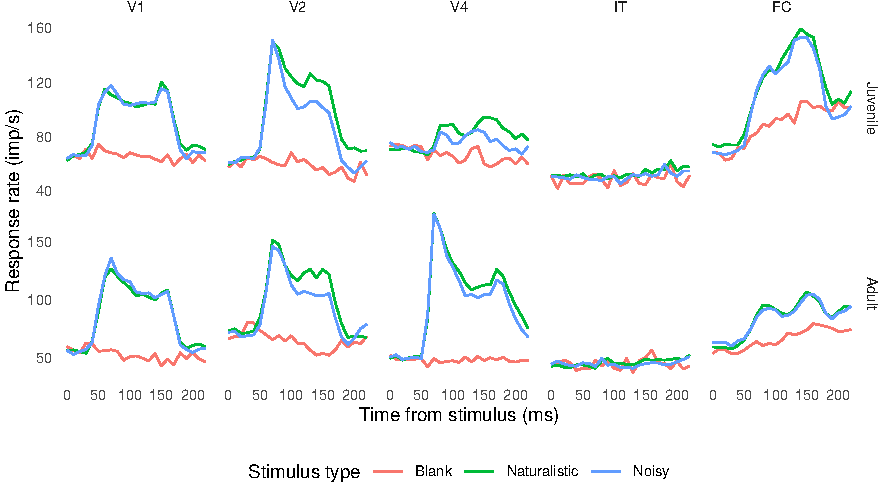
\includegraphics[keepaspectratio]{20260604_files/figure-pdf/fig-psth-1.pdf}}

}

\caption{\label{fig-psth}Averaged MUA for regions and the youngest
(juvenile) and oldest (adult) recording ages, which may differ by
region.}

\end{figure}%

\section{Visually responsive sites and onset
time}\label{visually-responsive-sites-and-onset-time}

Within the supplement of the main paper, Lee et al.~writes:

\begin{quote}
\emph{To determine whether a site was visually responsive in a given
recording session, we measured the average response separately for even
and odd repetitions of each stimulus. We measured the Pearson
correlation between these vectors, and used sites with a correlation of
0.4 or greater (the results reported here remained stable across a
variety of different metrics and thresholds)\ldots We defined the onset
time for a given site as the first deviation above a d' of ± 0.4, as
long as the following 2 windows were also suprathreshold (and of the
same sign). The onset time for a given population was the median onset
time across visually responsive sites. For most analyses, we then summed
responses across the 150 ms window following stimulus onset.}
\end{quote}

The \(d'\) referenced is Cohon's \(d\), calculated as \[
d' = \dfrac{\mu_1 - \mu_0}{\sqrt{(\sigma^2_1 + \sigma^2_0)/2}},
\] where contrasting blanks and stimuli provides the \(d'\) for
\emph{sensitivity} and contrasting noisy and naturalistic stimuli
provides the \(d'\) for \emph{selectivity}.

The procedure for finding onset site is a bit circular.

\begin{enumerate}
\def\labelenumi{\arabic{enumi}.}
\tightlist
\item
  Find a temporary onset time, with \(d'\) calculated between blanks and
  stimuli. The search window is 0 to 200 ms after stimulus presentation.
  If no onset time is found, use 100 ms as a placeholder.
\item
  Determine the responsive sites with signals averaged over a 150 ms
  window starting at the temporary onset time.
\item
  Find the onset time based on the responsive sites.
\end{enumerate}

For reference, see line 96 in
\texttt{repository\_textures2\_analysis\_figures\_v0.m}, which calls
\texttt{Textures2\_onset\_via\_discrim.m}. The responsive sites found
with the temporary onset time calculation can be seen in
Table~\ref{tbl-resp}. The final onset time is then calculated from only
the responsive sites and grouped by region and age, seen in
Table~\ref{tbl-onset}.

My results may differ from Lee et al.~because in Step 1, I calculate a
temporary onset time separated by array/subject. In contrast, Lee et
al.~performs all calculations after concatenating recordings from the
same region and age, which may contain up to three different arrays.

\begin{table}

\caption{\label{tbl-resp}Number of responsive sites found for each
region and age recorded, with arrays numbered arbitrarily.}

\centering{

\fontsize{9.0pt}{11.0pt}\selectfont
\begin{tabular*}{\linewidth}{@{\extracolsep{\fill}}rrrrr}
\toprule
Age (wks) & Array 1 & Array 2 & Array 3 & Total sites \\ 
\midrule\addlinespace[2.5pt]
\multicolumn{5}{l}{V1} \\[2.5pt] 
\midrule\addlinespace[2.5pt]
29 & {\cellcolor[HTML]{C9E4CF}{\textcolor[HTML]{000000}{21}}} & {\cellcolor[HTML]{999999}{\textcolor[HTML]{FFFFFF}{NA}}} & {\cellcolor[HTML]{999999}{\textcolor[HTML]{FFFFFF}{NA}}} & {\cellcolor[HTML]{C9E4CF}{\textcolor[HTML]{000000}{21}}} \\ 
37 & {\cellcolor[HTML]{C4E2CA}{\textcolor[HTML]{000000}{23}}} & {\cellcolor[HTML]{FFFFFF}{\textcolor[HTML]{000000}{0}}} & {\cellcolor[HTML]{999999}{\textcolor[HTML]{FFFFFF}{NA}}} & {\cellcolor[HTML]{C4E2CA}{\textcolor[HTML]{000000}{23}}} \\ 
56 & {\cellcolor[HTML]{A8D4B2}{\textcolor[HTML]{000000}{34}}} & {\cellcolor[HTML]{999999}{\textcolor[HTML]{FFFFFF}{NA}}} & {\cellcolor[HTML]{999999}{\textcolor[HTML]{FFFFFF}{NA}}} & {\cellcolor[HTML]{A8D4B2}{\textcolor[HTML]{000000}{34}}} \\ 
\midrule\addlinespace[2.5pt]
\multicolumn{5}{l}{V2} \\[2.5pt] 
\midrule\addlinespace[2.5pt]
29 & {\cellcolor[HTML]{CEE7D3}{\textcolor[HTML]{000000}{19}}} & {\cellcolor[HTML]{69B57E}{\textcolor[HTML]{000000}{58}}} & {\cellcolor[HTML]{999999}{\textcolor[HTML]{FFFFFF}{NA}}} & {\cellcolor[HTML]{2A9C56}{\textcolor[HTML]{FFFFFF}{77}}} \\ 
37 & {\cellcolor[HTML]{C9E4CF}{\textcolor[HTML]{000000}{21}}} & {\cellcolor[HTML]{81C091}{\textcolor[HTML]{000000}{49}}} & {\cellcolor[HTML]{999999}{\textcolor[HTML]{FFFFFF}{NA}}} & {\cellcolor[HTML]{45A565}{\textcolor[HTML]{FFFFFF}{70}}} \\ 
56 & {\cellcolor[HTML]{D6EBDA}{\textcolor[HTML]{000000}{16}}} & {\cellcolor[HTML]{8CC69A}{\textcolor[HTML]{000000}{45}}} & {\cellcolor[HTML]{999999}{\textcolor[HTML]{FFFFFF}{NA}}} & {\cellcolor[HTML]{60B177}{\textcolor[HTML]{FFFFFF}{61}}} \\ 
\midrule\addlinespace[2.5pt]
\multicolumn{5}{l}{V4} \\[2.5pt] 
\midrule\addlinespace[2.5pt]
29 & {\cellcolor[HTML]{9BCDA7}{\textcolor[HTML]{000000}{39}}} & {\cellcolor[HTML]{F7FBF8}{\textcolor[HTML]{000000}{3}}} & {\cellcolor[HTML]{999999}{\textcolor[HTML]{FFFFFF}{NA}}} & {\cellcolor[HTML]{94C9A0}{\textcolor[HTML]{000000}{42}}} \\ 
37 & {\cellcolor[HTML]{91C89E}{\textcolor[HTML]{000000}{43}}} & {\cellcolor[HTML]{D9ECDC}{\textcolor[HTML]{000000}{15}}} & {\cellcolor[HTML]{999999}{\textcolor[HTML]{FFFFFF}{NA}}} & {\cellcolor[HTML]{69B57E}{\textcolor[HTML]{000000}{58}}} \\ 
56 & {\cellcolor[HTML]{96CBA2}{\textcolor[HTML]{000000}{41}}} & {\cellcolor[HTML]{BADDC1}{\textcolor[HTML]{000000}{27}}} & {\cellcolor[HTML]{999999}{\textcolor[HTML]{FFFFFF}{NA}}} & {\cellcolor[HTML]{4BA869}{\textcolor[HTML]{FFFFFF}{68}}} \\ 
409 & {\cellcolor[HTML]{2A9C56}{\textcolor[HTML]{FFFFFF}{77}}} & {\cellcolor[HTML]{999999}{\textcolor[HTML]{FFFFFF}{NA}}} & {\cellcolor[HTML]{999999}{\textcolor[HTML]{FFFFFF}{NA}}} & {\cellcolor[HTML]{2A9C56}{\textcolor[HTML]{FFFFFF}{77}}} \\ 
\midrule\addlinespace[2.5pt]
\multicolumn{5}{l}{IT} \\[2.5pt] 
\midrule\addlinespace[2.5pt]
20 & {\cellcolor[HTML]{DEEFE1}{\textcolor[HTML]{000000}{13}}} & {\cellcolor[HTML]{999999}{\textcolor[HTML]{FFFFFF}{NA}}} & {\cellcolor[HTML]{999999}{\textcolor[HTML]{FFFFFF}{NA}}} & {\cellcolor[HTML]{DEEFE1}{\textcolor[HTML]{000000}{13}}} \\ 
31 & {\cellcolor[HTML]{FAFCFA}{\textcolor[HTML]{000000}{2}}} & {\cellcolor[HTML]{F5FAF6}{\textcolor[HTML]{000000}{4}}} & {\cellcolor[HTML]{FAFCFA}{\textcolor[HTML]{000000}{2}}} & {\cellcolor[HTML]{EBF5EC}{\textcolor[HTML]{000000}{8}}} \\ 
34 & {\cellcolor[HTML]{F5FAF6}{\textcolor[HTML]{000000}{4}}} & {\cellcolor[HTML]{FAFCFA}{\textcolor[HTML]{000000}{2}}} & {\cellcolor[HTML]{999999}{\textcolor[HTML]{FFFFFF}{NA}}} & {\cellcolor[HTML]{F0F7F1}{\textcolor[HTML]{000000}{6}}} \\ 
221 & {\cellcolor[HTML]{E3F1E6}{\textcolor[HTML]{000000}{11}}} & {\cellcolor[HTML]{999999}{\textcolor[HTML]{FFFFFF}{NA}}} & {\cellcolor[HTML]{999999}{\textcolor[HTML]{FFFFFF}{NA}}} & {\cellcolor[HTML]{E3F1E6}{\textcolor[HTML]{000000}{11}}} \\ 
\midrule\addlinespace[2.5pt]
\multicolumn{5}{l}{FC} \\[2.5pt] 
\midrule\addlinespace[2.5pt]
20 & {\cellcolor[HTML]{CEE7D3}{\textcolor[HTML]{000000}{19}}} & {\cellcolor[HTML]{999999}{\textcolor[HTML]{FFFFFF}{NA}}} & {\cellcolor[HTML]{999999}{\textcolor[HTML]{FFFFFF}{NA}}} & {\cellcolor[HTML]{CEE7D3}{\textcolor[HTML]{000000}{19}}} \\ 
31 & {\cellcolor[HTML]{F5FAF6}{\textcolor[HTML]{000000}{4}}} & {\cellcolor[HTML]{999999}{\textcolor[HTML]{FFFFFF}{NA}}} & {\cellcolor[HTML]{999999}{\textcolor[HTML]{FFFFFF}{NA}}} & {\cellcolor[HTML]{F5FAF6}{\textcolor[HTML]{000000}{4}}} \\ 
35 & {\cellcolor[HTML]{FFFFFF}{\textcolor[HTML]{000000}{0}}} & {\cellcolor[HTML]{999999}{\textcolor[HTML]{FFFFFF}{NA}}} & {\cellcolor[HTML]{999999}{\textcolor[HTML]{FFFFFF}{NA}}} & {\cellcolor[HTML]{FFFFFF}{\textcolor[HTML]{000000}{0}}} \\ 
\bottomrule
\end{tabular*}

}

\end{table}%

\begin{table}

\caption{\label{tbl-onset}Calculated onset times, when responsive sites
are grouped by region and age. FC at 35 weeks has no responsive sites
and therefore defaults to an onset of 100 ms in future calculations. The
last column reports the proportion of sites where an onset was found.}

\centering{

\fontsize{9.0pt}{11.0pt}\selectfont
\begin{tabular*}{\linewidth}{@{\extracolsep{\fill}}rrrrrr}
\toprule
Age (wks) & Onset time (ms) & Min. onset & Max. onset & Responsive sites & Prop. with onset \\ 
\midrule\addlinespace[2.5pt]
\multicolumn{6}{l}{V1} \\[2.5pt] 
\midrule\addlinespace[2.5pt]
29 & {\cellcolor[HTML]{C9E4CE}{\textcolor[HTML]{000000}{40}}} & 60 & 70 & 21 & {\cellcolor[HTML]{4682B4}{\textcolor[HTML]{FFFFFF}{1.00}}} \\ 
37 & {\cellcolor[HTML]{C9E4CE}{\textcolor[HTML]{000000}{40}}} & 60 & 70 & 23 & {\cellcolor[HTML]{5087B7}{\textcolor[HTML]{FFFFFF}{0.957}}} \\ 
56 & {\cellcolor[HTML]{C9E4CE}{\textcolor[HTML]{000000}{40}}} & 60 & 80 & 34 & {\cellcolor[HTML]{4682B4}{\textcolor[HTML]{FFFFFF}{1.00}}} \\ 
\midrule\addlinespace[2.5pt]
\multicolumn{6}{l}{V2} \\[2.5pt] 
\midrule\addlinespace[2.5pt]
29 & {\cellcolor[HTML]{ADD6B6}{\textcolor[HTML]{000000}{60}}} & 60 & 130 & 77 & {\cellcolor[HTML]{4984B5}{\textcolor[HTML]{FFFFFF}{0.987}}} \\ 
37 & {\cellcolor[HTML]{ADD6B6}{\textcolor[HTML]{000000}{60}}} & 60 & 80 & 70 & {\cellcolor[HTML]{4682B4}{\textcolor[HTML]{FFFFFF}{1.00}}} \\ 
56 & {\cellcolor[HTML]{ADD6B6}{\textcolor[HTML]{000000}{60}}} & 70 & 130 & 61 & {\cellcolor[HTML]{4A84B5}{\textcolor[HTML]{FFFFFF}{0.984}}} \\ 
\midrule\addlinespace[2.5pt]
\multicolumn{6}{l}{V4} \\[2.5pt] 
\midrule\addlinespace[2.5pt]
29 & {\cellcolor[HTML]{A0CFAA}{\textcolor[HTML]{000000}{70}}} & 80 & 170 & 42 & {\cellcolor[HTML]{6E98C2}{\textcolor[HTML]{FFFFFF}{0.810}}} \\ 
37 & {\cellcolor[HTML]{76BB88}{\textcolor[HTML]{000000}{100}}} & 80 & 150 & 58 & {\cellcolor[HTML]{B3C7DF}{\textcolor[HTML]{000000}{0.431}}} \\ 
56 & {\cellcolor[HTML]{A0CFAA}{\textcolor[HTML]{000000}{70}}} & 70 & 140 & 68 & {\cellcolor[HTML]{ACC2DC}{\textcolor[HTML]{000000}{0.471}}} \\ 
409 & {\cellcolor[HTML]{ADD6B6}{\textcolor[HTML]{000000}{60}}} & 70 & 80 & 77 & {\cellcolor[HTML]{4984B5}{\textcolor[HTML]{FFFFFF}{0.987}}} \\ 
\midrule\addlinespace[2.5pt]
\multicolumn{6}{l}{IT} \\[2.5pt] 
\midrule\addlinespace[2.5pt]
20 & {\cellcolor[HTML]{349F5B}{\textcolor[HTML]{FFFFFF}{140}}} & 160 & 160 & 13 & {\cellcolor[HTML]{F2F5F9}{\textcolor[HTML]{000000}{0.0769}}} \\ 
31 & {\cellcolor[HTML]{67B47C}{\textcolor[HTML]{000000}{110}}} & 120 & 150 & 8 & {\cellcolor[HTML]{BDCEE3}{\textcolor[HTML]{000000}{0.375}}} \\ 
34 & {\cellcolor[HTML]{84C293}{\textcolor[HTML]{000000}{90}}} & 110 & 170 & 6 & {\cellcolor[HTML]{89AACD}{\textcolor[HTML]{000000}{0.667}}} \\ 
221 & {\cellcolor[HTML]{84C293}{\textcolor[HTML]{000000}{90}}} & 110 & 110 & 11 & {\cellcolor[HTML]{EFF3F8}{\textcolor[HTML]{000000}{0.0909}}} \\ 
\midrule\addlinespace[2.5pt]
\multicolumn{6}{l}{FC} \\[2.5pt] 
\midrule\addlinespace[2.5pt]
20 & {\cellcolor[HTML]{A0CFAA}{\textcolor[HTML]{000000}{70}}} & 70 & 130 & 19 & {\cellcolor[HTML]{4682B4}{\textcolor[HTML]{FFFFFF}{1.00}}} \\ 
31 & {\cellcolor[HTML]{92C99F}{\textcolor[HTML]{000000}{80}}} & 70 & 120 & 4 & {\cellcolor[HTML]{4682B4}{\textcolor[HTML]{FFFFFF}{1.00}}} \\ 
35 & {\cellcolor[HTML]{999999}{\textcolor[HTML]{FFFFFF}{NA}}} & NA & NA & 0 & {\cellcolor[HTML]{FFFFFF}{\textcolor[HTML]{000000}{0}}} \\ 
\bottomrule
\end{tabular*}

}

\end{table}%

\section{Averaged responses}\label{averaged-responses}

The responsive sites and onset times produce the time-averaged matrices
of the responses. I grouped measurements by region and age, i.e.,
removing the distinction between subjects, and averaged responses in a
150 ms window.




\end{document}
